\section{Course syllabus}
\subsection{Course Objective}
This course is designed to introduce a student with a reasonable understanding of
biology to the basic techniques of mathematical modeling. Specifically, the student
will be able to take a conceptual model of some biological system and transform it
into an appropriate mathematical framework. The student will also be able to develop
intuition based on their model and to interpret simulation results to draw conclusions.

\subsection{Course Design}

\paragraph{Content, Converse, Convey}
For each lesson in the course, the assignments will proceed in three parts. First,
students will familiarize themselves with the content of that week’s lesson and take a
short quiz to ensure that they have done the necessary reading. Second, the
students will meet in class or use the online forum to converse on a problem related
to the lesson. Finally, ever student will be given their own related problem to solve
and convey their answer on our class wiki for other students to evaluate.

\paragraph{Programming Projects}
In addition to the weekly assignments, the students will also be synthesizing their
knowledge of mathematical modeling concepts to build their own simple modeling
projects. By the third week the students will be able to pick a biological system to
study. They will work during a few of the hour long discussions to put together their
own model of the system and explain it to the rest of the class. Finally, they will
present an in-depth description of their project on the class wiki.

\subsection{Assignments}
\paragraph{Readings and Quizzes}
There are readings and lectures online for you to become introduced to the material
before you come to class. There will be online quizzes on Chalk which will be due by
Tuesday at midnight the day before new material is covered in class. These quizzes
should resemble simple multiple choice exam questions; they merely check whether
you have viewed the material. However, in total these quizzes count towards 25% of
your overall grade so take them seriously.

\paragraph{Class Forum Discussions}
Every week, the class will meet together to tackle a problem related to the lesson.
The problems are frequently posed based on questions left unanswered by studentsin the previous year. The class should come to a reasonable consensus by the end of the session or they should follow up online to come to an agreement. I’ve designed the discussion sections so that you don’t need to be the most boisterous student to participate in the discussion meaningfully. There will be an
equal weight to valuable comments given in person as well as those on our online forum. In addition, our class discussions will often contain smaller discussions that allow for one-on-one interaction. Nevertheless, class discussion accounts for 25\% of
your grade so, whether in the forums or in person, your participation is required.

\paragraph{Wiki Articles}
Each student will be given a more in-depth problem for each lesson to be written up
and posted to the group wiki. Here we are not just looking for a solution to the
problem. We need an explanation of your approach and why it is right. Your peers will
be evaluating your work to make sure that it makes sense to them. The writing and
evaluation of these assignments will count for another 25\% of your grade.

\paragraph{Final Project}
By the third week of this course, the student should start to have an understanding of
what types of systems can be modeled with a differential equation. At this point in
time, the students will select a biological system to model as their final project. The
class during 4th week will involve every student briefly stating their problem area how
they will model it.  Please note that the system you are modeling does not
have to be extremely complex, and the model you generate does not have to be
perfectly accurate. The goal of this project is simply to show that you understand all
of the steps in moving from an abstract idea to a mathematical model. By the end of
the session you should have a reasonably involved computational model.



\section{Post-class Student Survey}

I asked the students to give me some feedback on their experience in the course and what could be improved.  Feedback was generally positive and instructive in looking for ways to improve.

\begin{figure}[h!]
	\centering
	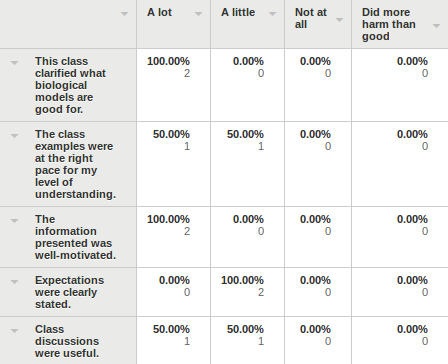
\includegraphics[width=0.8\hsize]{workshop/table_of_responses.png}
	\caption{Responses from student survey.  Only 2 of 5 students replied.} 
	
\end{figure}

\paragraph{What are some questions you have about biological modeling that this class should have addressed.}

I think it might be good to emphasize presentation and interpretation of modeling results, both from the perspective of the experimenter and the reader. In other words, I think it would be good for people to become comfortable both reading theoretical papers and generating simple modeling figures. I know this wasn't the focus of the workshop, but it might be nice to briefly cover agent-based modeling to the point where someone could be conformable interpreting experiments. 

It was a good foundation. Maybe how to interpret a model in a paper and evaluate it, if we did an example in class that would be helpful. 

\paragraph{ Describe how you would like to see this workshop structured to best promote your learning of the material }

It might be a good idea to have a list of things to model, so that people can still progress through the workshop even if the system they work on isn't amenable to modeling or isn't interesting to model. I liked the emphasis on students giving short presentations throughout. 

A little more background on the basic calculus we needed. Also talking more about the reasoning behind what you're doing and less algebra on the board, it's kinda hard to follow but we can all probably do it. 




\section{Reflections and Future Ideas}

In general, the students reacted positively to the framework that we established with it's emphasis on the three C's outlined above.  The student survey responses showed that the focus on classroom participation was welcome.  In practice, the students were not required to complete any homework, and the course was not given for a grade.  This led to many of the assignments being neglected entirely.  However, despite all of the work being completely optional, many of the students completed a significant portion of the work voluntarily.  

In the future, I will need to do a bit more preparation work to select a larger corpus of example systems for students to work with.  And having more examples to work through together will also probably improve outcomes. On the other hand, I don't want to lose the student driven focus that I was hoping to attain. I may also want to establish a bit more authority so that students attend class with their assignments completed.   


\section{Course Materials}

The course slides are available online at the following URL:

https://drive.google.com/drive/folders/0B3gBL61483U8Z2h1b3JRUHZMQ1k?usp=sharing

Below you can find the Q\&A material used for quizzes or discussion prompts.


\subsection{How mathematical models make sense of complex processes}

% 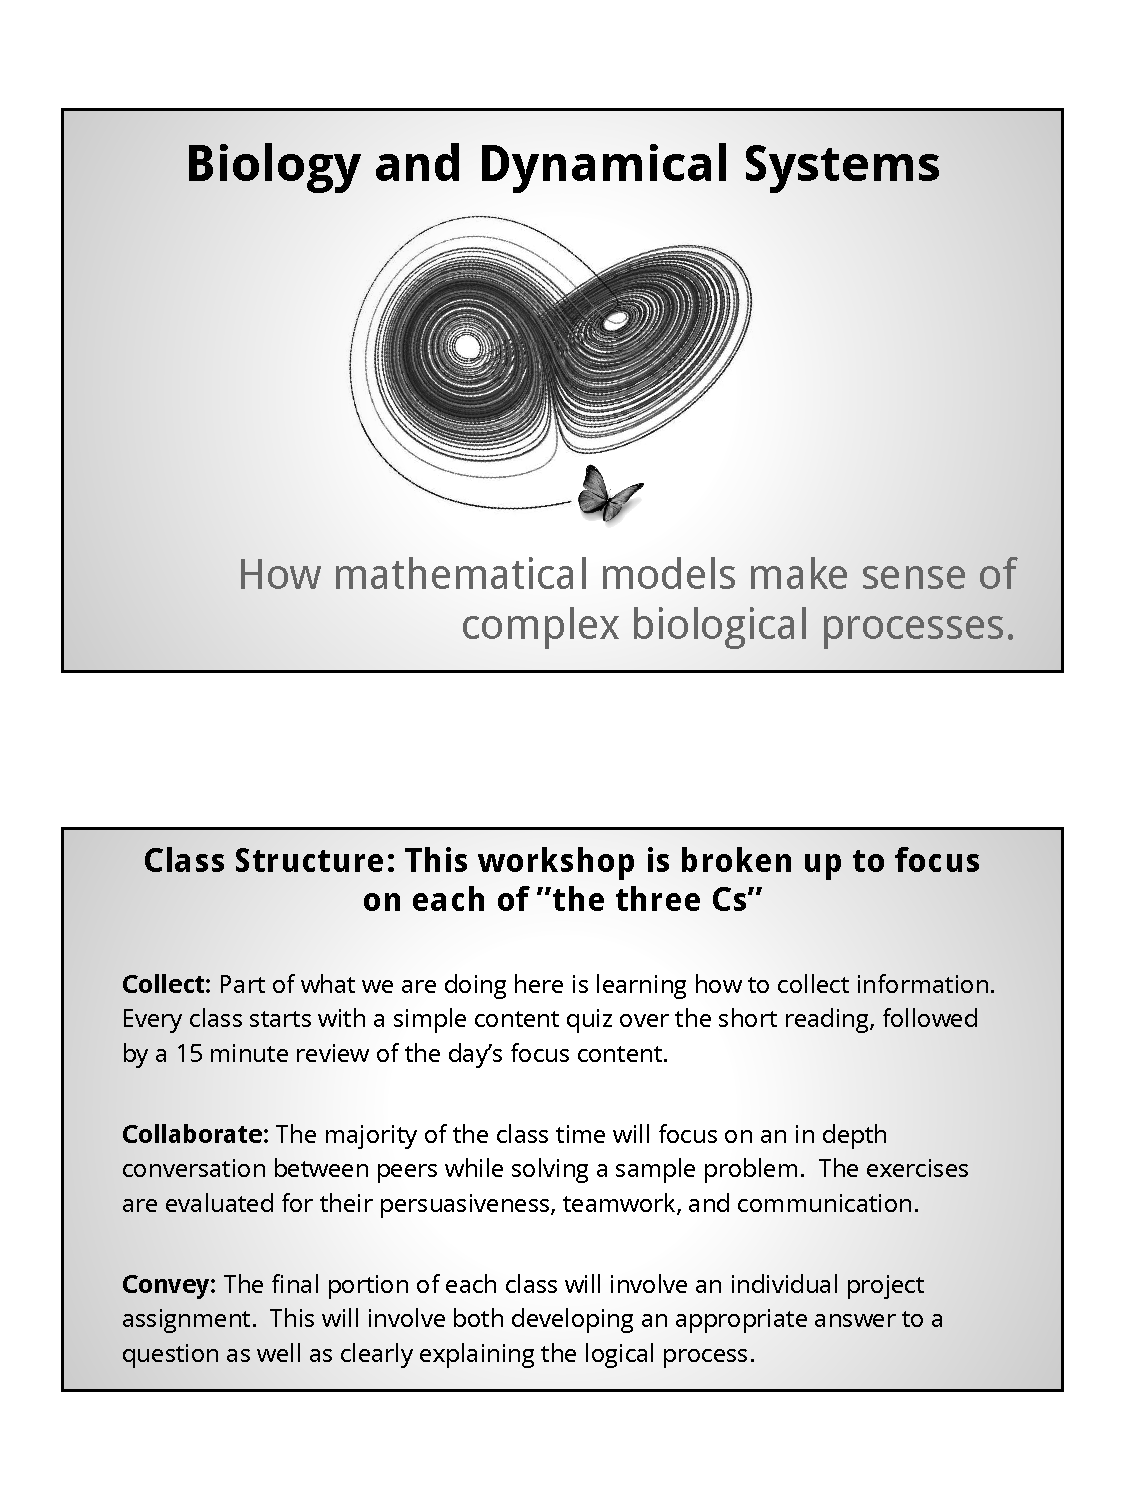
\includepdf[pages={1-}]{workshop/wk1_intro_and_cartoons.pdf}


\subsection{Modeling biological systems with differential equations}
\paragraph{Modelling biological systems} is a significant task of systems biology and mathematical biology. It involves the use of computer simulations of biological systems, including cellular subsystems (such as the networks of metabolites and enzymes which comprise metabolism, signal transduction pathways and gene regulatory networks), to both analyze and visualize the complex connections of these cellular processes.'' --Wikipedia

\paragraph{Many types of models} Biological models can work in many different ways:  In general, models are made to focus on systems at a certain scale.  We can choose from a wide variety of model types. Some work by modeling continuous values, such as concentration of a protein.  Others work by modeling the discrete state of a system, such as a neuron being either on or off.  Some models are deterministic, meaning that there is no randomness, while others add stochastic noise.

\paragraph{Focusing on Differential equations} In our class we?re going to focus on probably the simplest and most widely used kind of mathematical model, differential equations.  Differential equations are a continuous, deterministic model, they model real values with rules that describe exactly how those values change.  Differential equations are very similar to the equations we learned about in our high school and college calculus courses.

\paragraph{What is a differential equation good for?} A differential equation is a simple formula that describes how a system will change in time based on the state of the system right now. You can think of it like a very formal protocol for how concentrations of substances will change over time.  For example, a differential equation 

% 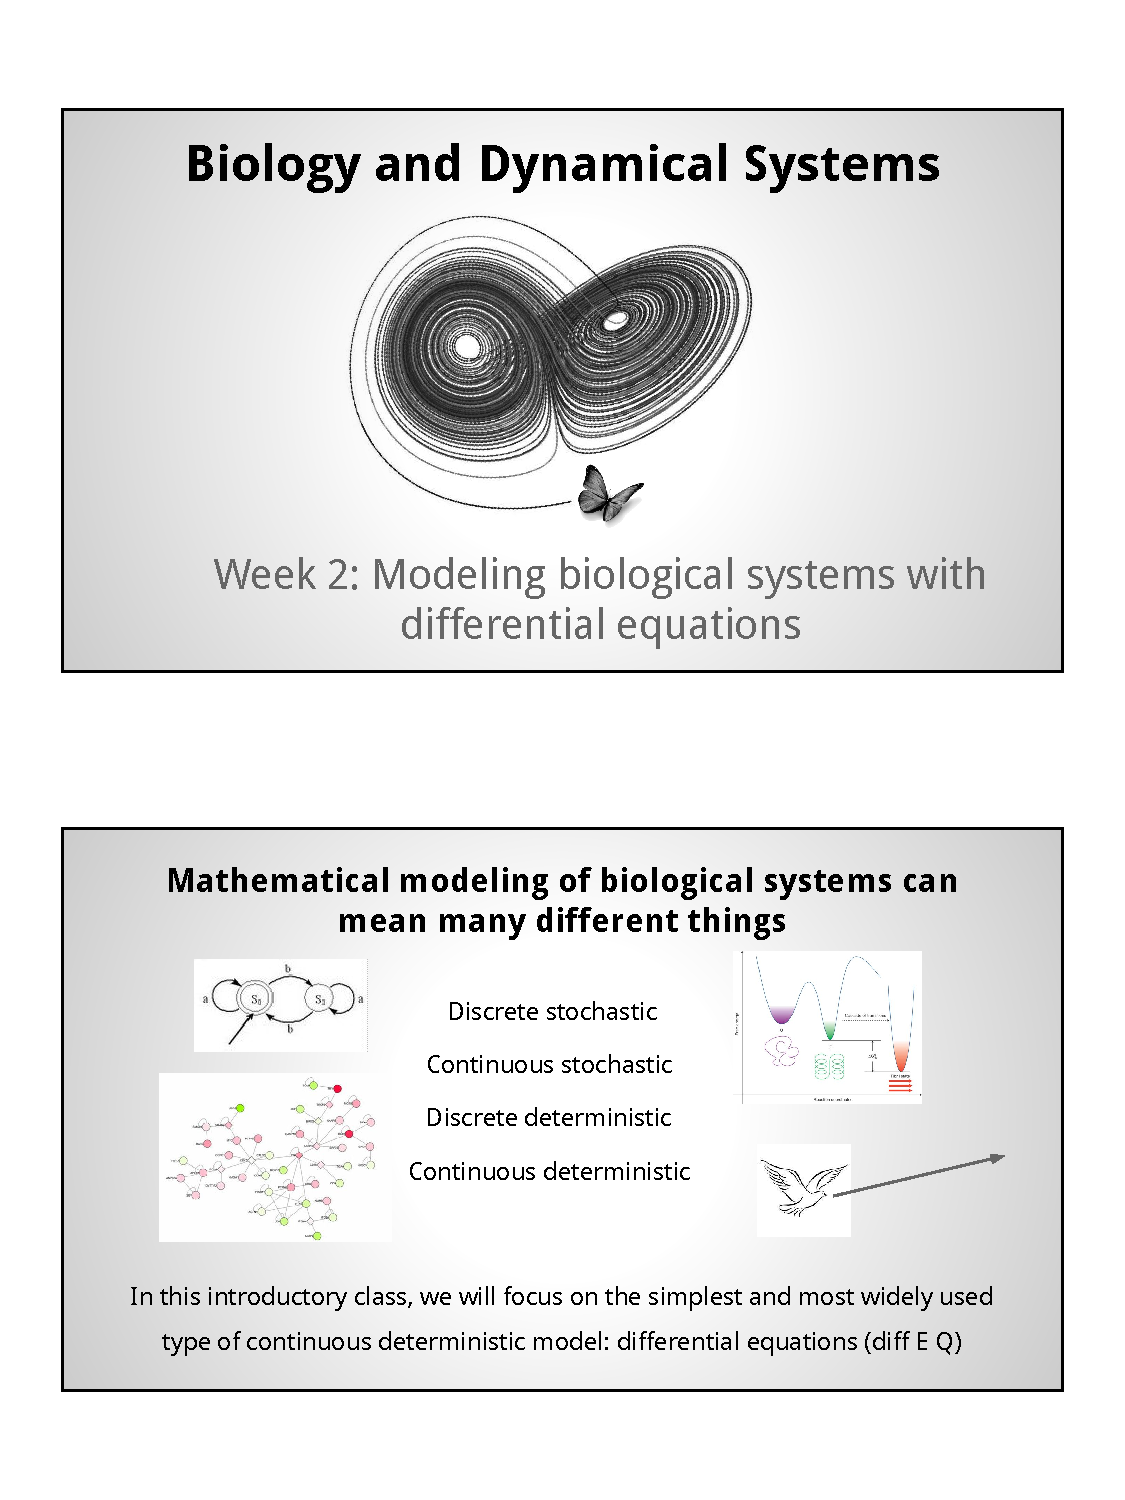
\includepdf[pages={1-}]{workshop/wk2_diff_eq.pdf}



\subsection{Visualizing equations with graphs}
\paragraph{Why is it called differential?} One could argue that differential equations could actually be called derivative equations.  That?s because the equation itself is really just a way of explicitly writing out the derivative of a variable.  For those that don?t remember a derivative is just ?a way to represent rate of change, that is - the amount by which a function is changing at one given point...it is the slope of the tangent line at a point on a graph.?

\paragraph{Equilibrium?} Another important concept in diffeq is that of equilibrium.  The meaning of equilibrium is simple once you have a rate equation to look at.  When the net rates of change of all variable are equal to 0, then nothing can change anymore.  The rates of production and destruction are balanced, and the concentrations of everything will remain constant forever.  Not all systems reach equilibrium, but most do, and finding equilibria is the first step to understanding how many systems work.  We will use equilibrium and steady state more or less interchangeably though there are subtle, pedantic differences.

\paragraph{Initial conditions and transient behaviors} Even though most systems reach equilibrium after a long time, the system?s initial conditions set the early ?transient? behavior. The initial condition, or seed value, is simply the state of the system where we choose to start.  The transient behavior is the way in which the system changes from the initial conditions to the steady state.

\paragraph{What are nullclines?} If our rate equation has two variables that can change in it (i.e. not constants), then there is no longer a single value at which the rate equation will equal 0.  Instead there will be a set of values that make the rate 0.  This set of values defines a line, and this line is called a nullcline. 
% 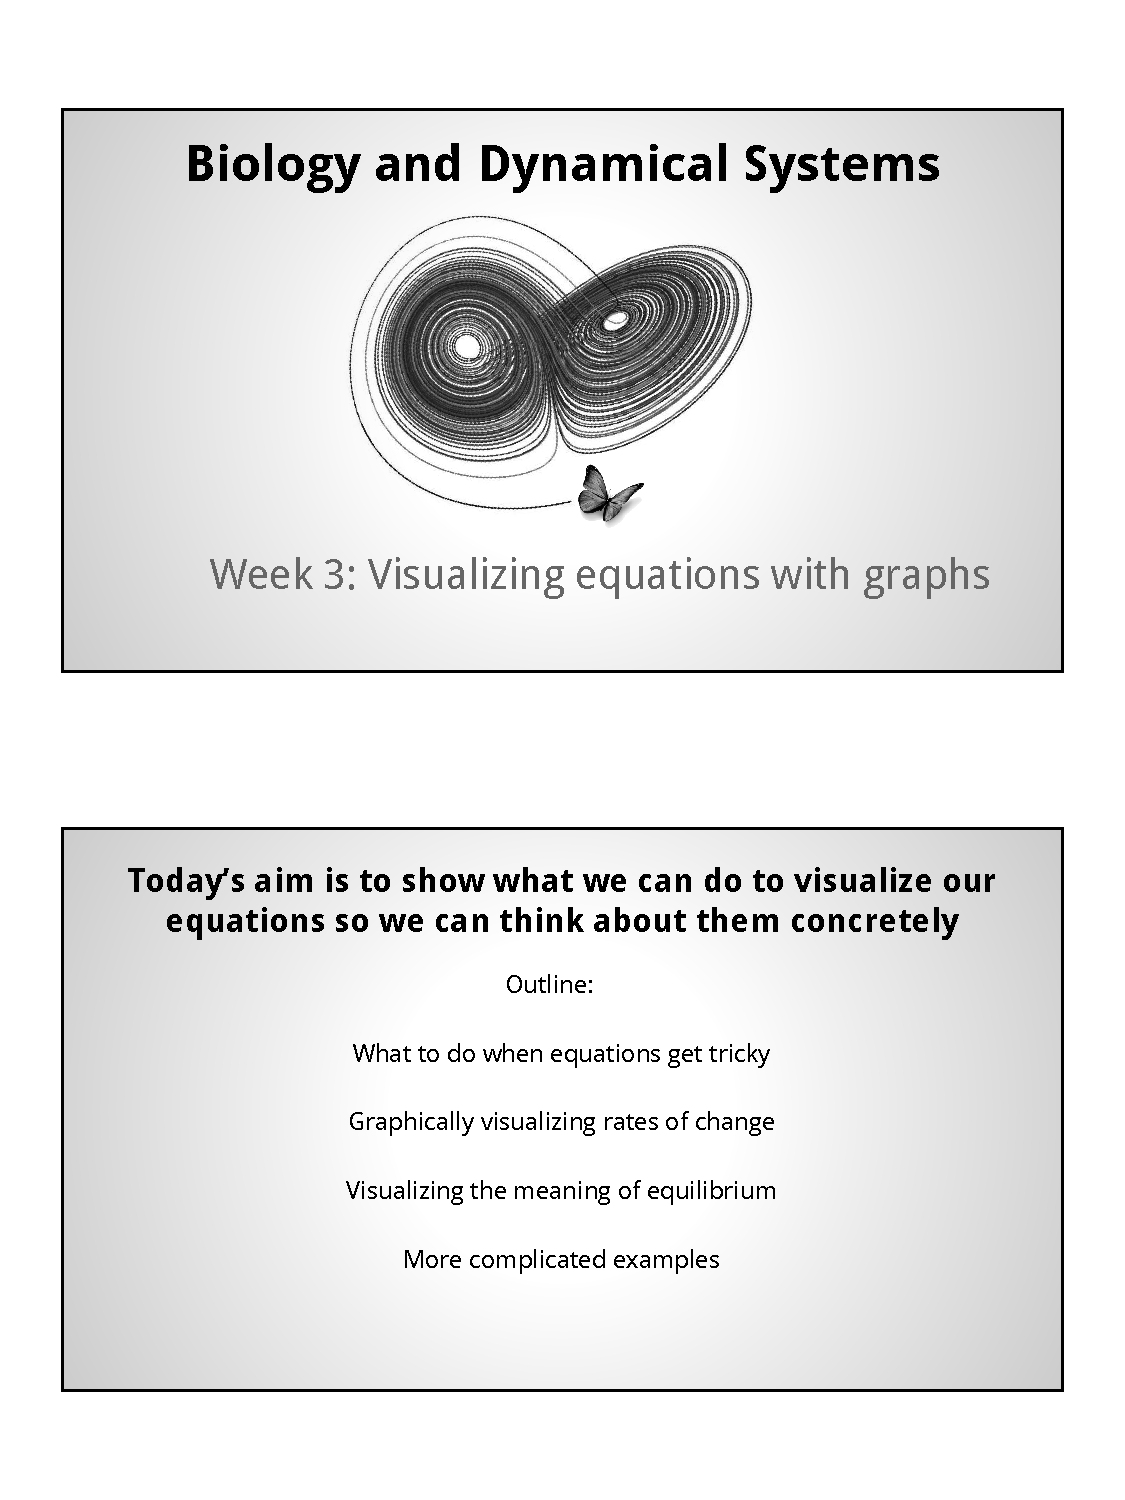
\includepdf[pages={1-}]{workshop/wk3_diag.pdf}



\subsection{Simplifying models and starting simulations}
\paragraph{Why simplify before simulating?} There are a number of reasons to simplify your equations before you ever start a simulation.  Here are my top three.  
1) You won?t be able to remember or adequately describe all the parameters that went into a given simulation when somebody asks you.  If you have 20 parameters in a simulation there will always be a huge risk that you screwed one of them up and you will never be able to notice.  
2) If you want to understand how your model works under many different conditions, then every time you add a parameter you have to do exponentially more work.  In other words, when you are systematically checking how 3 parameters work together you may have to do $100^3$ different simulations and analyze your results.  If you add one more parameter you will have to do $100^4$ simulation or 100 times more work.  
3) Nobody wants to look at a disorganized giant equation.  If you have a complicated equation most people will decide it isn?t worth their time to pay attention to the modeling so none of your modeling work will count for anything anyway.

\paragraph{The parts of a differential equation model} A differential equation model can be broken down into 3 parts: variables, parameters, and the form of the equation.  Variables are the values (like concentration) that are changing in time.  This is the physically ?real? stuff like the number of proteins or the size of your cell.  Parameters are things like rate constants and diffusion coefficients.  These are descriptive numbers that set the magnitudes of rates of change.  Finally, the form of the equation determines how the variables and parameters fit together.  This is the level at which we can see how each variable affects the other qualitatively, but it takes parameters to know by how much.

\paragraph{How do simulations work?} The applied math behind solving differential equations with computers is rich and we certainly won?t understand everything that has been done over the past 70 years to solve these problems.  However we can get some intuition by looking at the simplest way of solving, called the Euler method.  In this method you ?step? through time and change the value of your variables by a small amount using the rules defined in your differential equation (See wikipedia page for more info).  If you ever try this, you will get bored very fast because it is really annoying.  But when computers do this, they can take very small steps and therefore ?solve? the system with arbitrary accuracy.  There have been a bunch of modifications of this technique that significantly improve the accuracy vs timestep tradeoff.


% 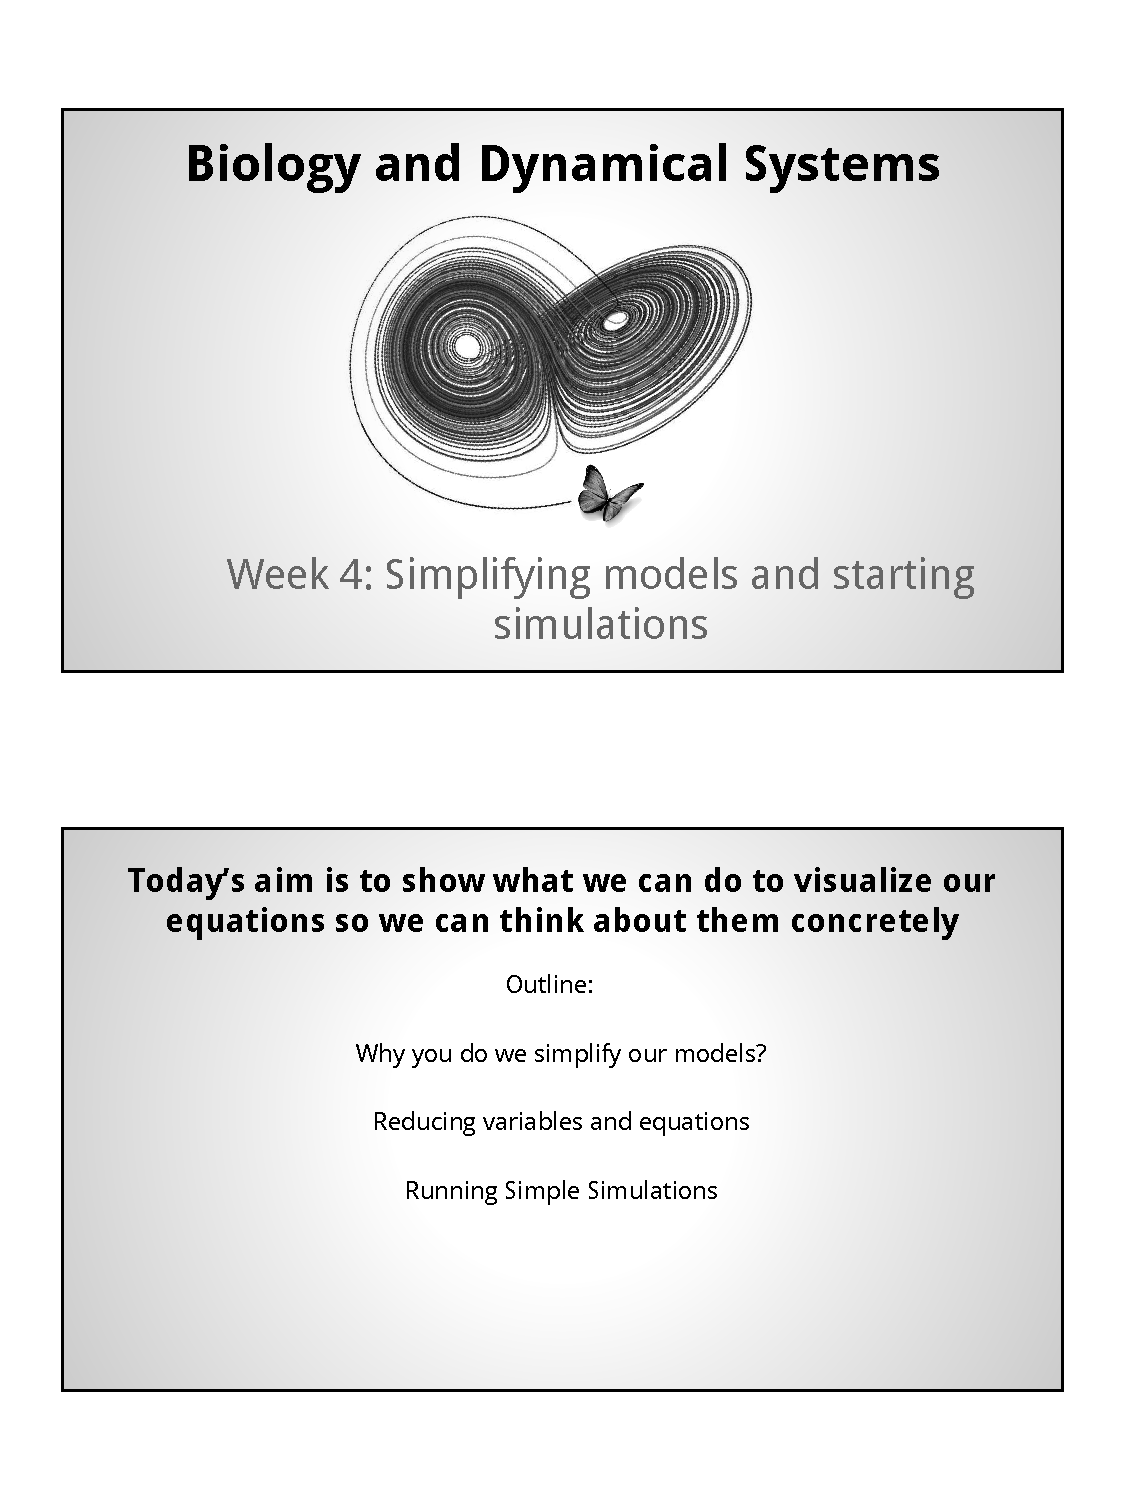
\includepdf[pages={1-}]{workshop/wk4_simple.pdf}



\subsection{Analyzing equations and understanding simulation output}

\paragraph{(from wikipedia) Nondimensionalization} is the partial or full removal of units from an equation involving physical quantities by a suitable substitution of variables. This technique can simplify and parameterize problems where measured units are involved. It is closely related to dimensional analysis. In some physical systems, the term scaling is used interchangeably with nondimensionalization, in order to suggest that certain quantities are better measured relative to some appropriate unit. These units refer to quantities intrinsic to the system, rather than units such as SI units. Nondimensionalization is not the same as converting extensive quantities in an equation to intensive quantities, since the latter procedure results in variables that still carry units.

\paragraph{Running simulations}: The following two snippets of code is all you need to solve differential equations in MATLAB.


\begin{verbatim}
function dc = myode(t,p,a,b)
    p1 = p(1);
    p2 = p(2);
    dp1 = 1 - a*p2 - p1;
    dp2 =p1 - b*p2;
    dp = [dp1;dp2];
end
\end{verbatim}

\begin{verbatim}
t = 0:0.1:10;      #timepoints for solution (1 to 10 increment of 0.1)
p0 = [1,0];         #initial conditions for the concentration of p1 and p2
a=1; b=1;          #optional constants a and b which will change behavior
[t, pt] = ode45(@myode,t,p0,[],a,b);        #this runs the simulaton 
plot(t,p(:,1)); hold on; plot(t,p(:,2));           #this plots the output
\end{verbatim}

So now you can put whatever you want into the equation and change your parameters and run many simulations.  

% 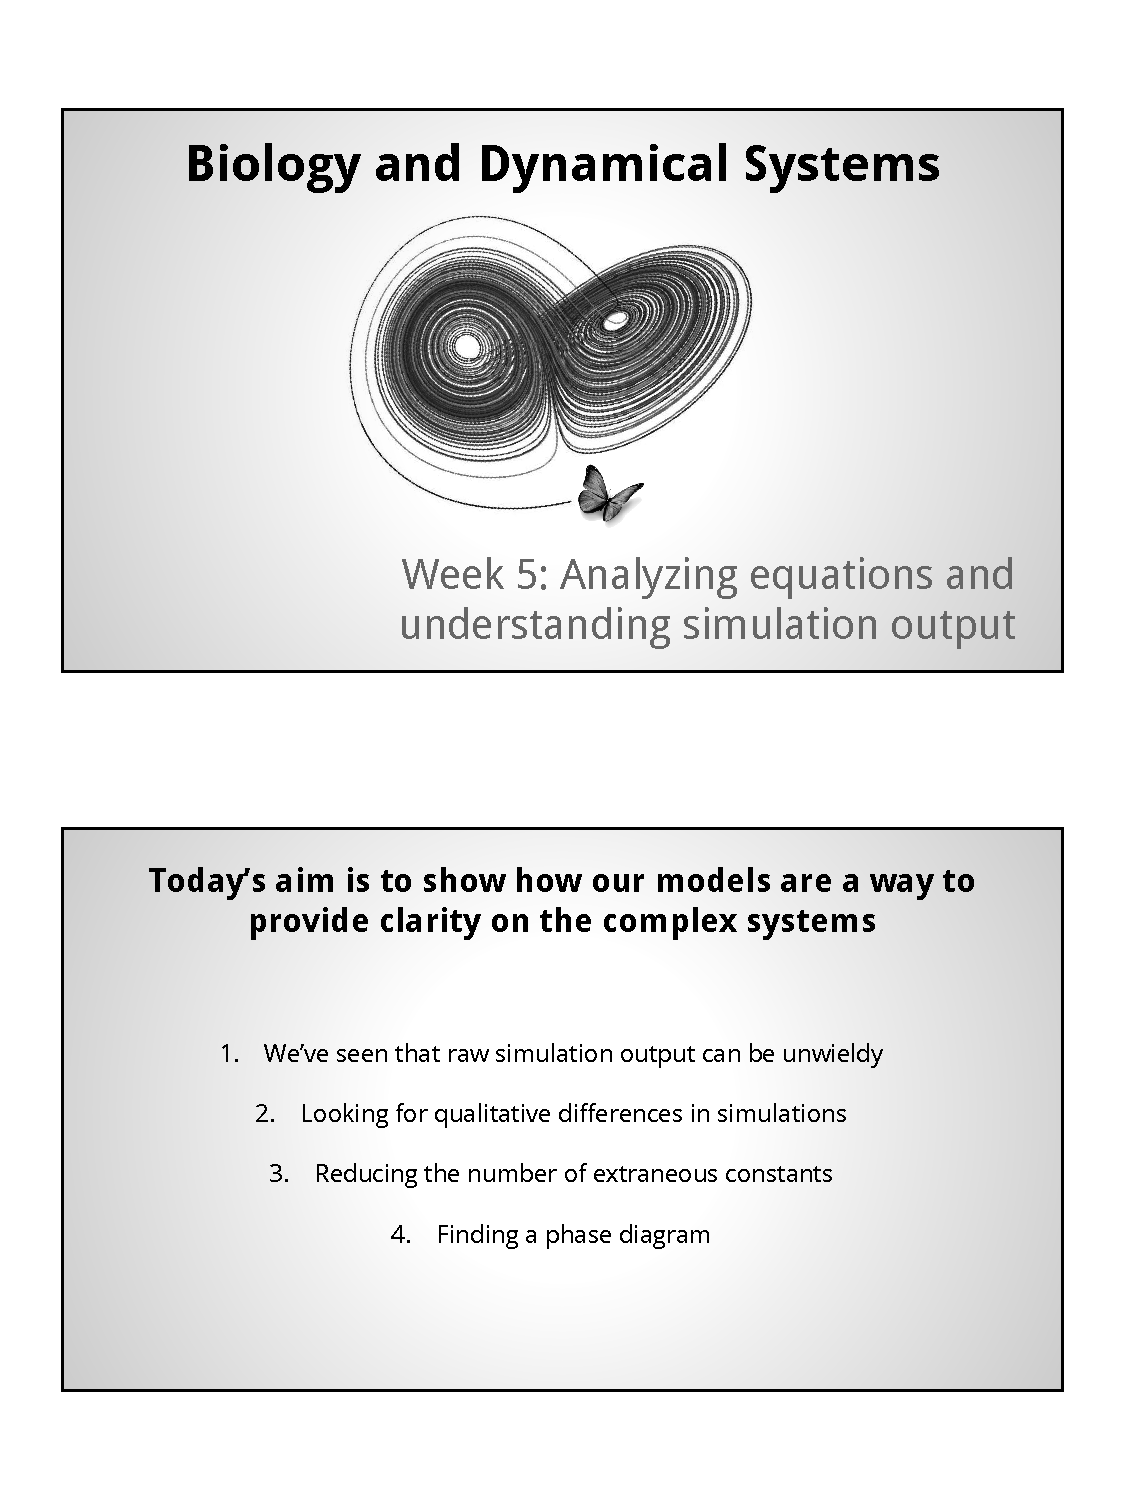
\includepdf[pages={1-}]{workshop/wk5_analysis.pdf}



\subsection{Explaining ever more complex systems}

% 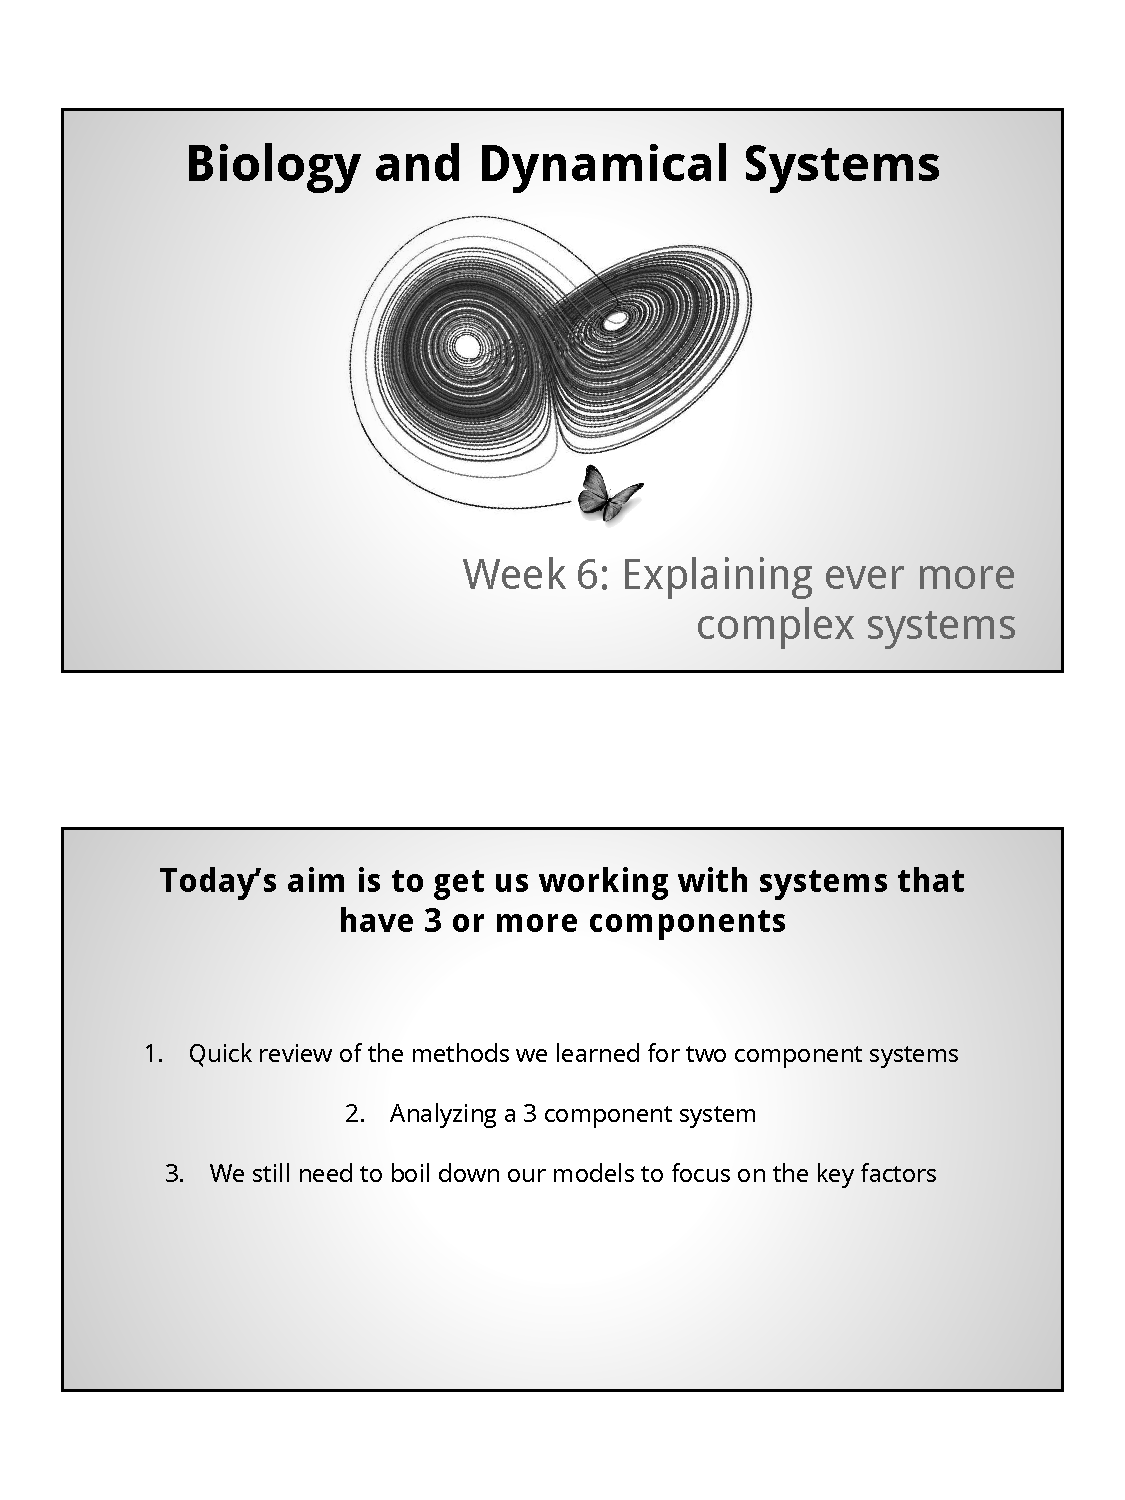
\includepdf[pages={1-}]{workshop/wk6_display.pdf}


\section{Quizzes and Project ideas}
\paragraph{W2}
Q1: Which is not a situation that is amenable to mathematical modeling?
A metabolism, signal transduction pathways, gene regulatory networks, protein purification

Q2: Which is a category of biological mathematical model?
A soft, prescient, discrete, topological

Q3: Which type of model is a differential equation?
A continuous deterministic, discrete stochastic, continuous stochastic, discrete deterministic

Q4: What does a differential equation most closely resemble?
A a protocol, a patent, a dissertation, a legume


\paragraph{W3}
Q1: Which is the closest synonym for derivative in the context of diffeq?
A Unoriginal, by-product, change, sum

Q2: Which is least similar to equilibrium?
A balanced rates, constant concentrations, discrete probabilities, steady states

Q3: Which conditions set the transient behavior?
A initial, parametric, hyperbolic, final

Q4: Nullclines are...
A topographical, unimportant, lines, esoteric

\paragraph{W4}
Q1: Number of simulations to run varies --- with the number of free parameters.
A quadratically, logarithmically, exponentially, combinatorially

Q2: Which is not a part of a differential equation model?
A definitions, variables, parameters, the form of the equation

Q3:The Euler method gives exact solutions.
A True, False, neither, depends who you ask

Q4: Who likes looking at a disorganized mess of an equation?
A Your PI, your colleagues, your reviewer, nobody

\paragraph{W5}
Q1: Once nondimensionalization is complete?
A All variables have units of time, there are no more parameters left, equations are simpler to analyze, your solutions will fall on a line

Q2: In MATLAB --- is the function for solving differential equations
A ode23tb, ode113, ode45, ode15i

Q3: Which isn?t necessary to solve a differential equation
A An ode function, constants, initial conditions, timepoints for solution
